\PassOptionsToPackage{sols}{handout}
\documentclass[main]{subfiles}
\setcounterrefbeforedot{chapter}{m-ws2-2}
\setcounterrefafterdot{section}{m-ws2-2}
\addtocounter{section}{-1}
\usepackage{solutions}

\begin{document}

\ifSubfilesClassLoaded{%
  \chaptermark{\chaptertwo}
}{}

\section{The Unit Circle, Sine and Cosine} \label{ws2-2}

% \begin{objectives}

% Learning Objectives:

% \begin{itemize}[topsep=0pt,partopsep=0pt,parsep=8pt,itemsep=0pt]

% \item You should understand the definition of $\tan x$ and its unit circle
%   interpretation as the slope of the line between the origin and $P(x)$. 

% \item You should understand the graph of $\tan x$ and its connection with
%   the graphs of $\sin x$ and $\cos x$.

% \item You should be comfortable using both radians and degrees to describe
%   angles.

% \item You should understand the relationship between angles and arc
%   length (by ``arc length,'' we mean the length of an arc of a circle).

% \item You should be able to use symmetry and the unit circle to reason
%   about trigonometric values of related angles.  (For example, you should
%   be able to determine how $\sin(\pi - x)$ relates to $\sin x$.)

% \end{itemize}
% \end{objectives}

\textbf{Key Idea}: The unit circle has a radius of 1 unit, making it easy to scale up or down as needed.

\begin{enumerate}

\item
\begin{problem}
    On your homework, you used the special right triangles to find the coordinates of points on the circle of radius 1 centered at the origin. We will use these coordinates often, so practice recalling them, as well as the associated angles in radians.
\end{problem}
\begin{center}
\begin{tabular}{cc}

\begin{tikzpicture}
      
  \begin{axis}[
  xmin=-1.1, xmax=1.1,
  ymin=-1.1, ymax=1.1,
  xlabel=\large$x$, ylabel=\large$y$,
  xtick=\empty, ytick=\empty,
  axis equal = true
  ]
  \coordinate (O) at (0,0);
  \coordinate (X) at (1,0);
  \coordinate (Y) at (0,1);
  \addplot[domain=0:360, data cs=polar] (x,1);
  \end{axis}
  \begin{scope}[x={($(X)-(O)$)}, y={($(Y)-(O)$)}, shift={(O)}]
    \foreach \A in {0,90,180,270} {
      \filldraw[radius=2pt] (\rtheta{1}{\A}) circle;
    }
    \foreach \A in {45, 135, 225, 315} {
      \filldraw[radius=2pt] (\rtheta{1}{\A}) circle;
    }
        \solonly{
    \node[above right] at (0:1) {$(1,0)$};
    \node[above right] at (45:1) {$\big(\frac{\sqrt{2}}{2},\frac{\sqrt{2}}{2}\big)$};
    \node[above right] at (90:1) {$(0,1)$};
    \node[above left] at (135:1) {$\big({-\frac{\sqrt{2}}{2}},\frac{\sqrt{2}}{2}\big)$};
    \node[below left] at (180:1) {$(-1,0)$};
    \node[below left] at (225:1) {$\big({-\frac{\sqrt{2}}{2}},{-\frac{\sqrt{2}}{2}}\big)$};
    \node[below right] at (270:1) {$(0,{-1})$};
    \node[below right] at (315:1) {$\big(\frac{\sqrt{2}}{2},{-\frac{\sqrt{2}}{2}}\big)$};
    }
    \solonly{
    \node[above left] at (0:1) {$0$};
    \node[below left] at (45:1) {$\pi/4$};
    \node[below] at (90:1) {$\pi/2$};
    \node[below right] at (135:1) {$3\pi/4$};
    \node[below right] at (180:1) {$\pi$};
    \node[above right] at (225:1) {$5\pi/4$};
    \node[above] at (270:1) {$3\pi/2$};
    \node[above left] at (315:1) {$7\pi/4$};
    }
  \end{scope}
  
\end{tikzpicture}

&
\begin{tikzpicture}
      
  \begin{axis}[
  xmin=-1.1, xmax=1.1,
  ymin=-1.1, ymax=1.1,
  xlabel=\large$x$, ylabel=\large$y$,
  xtick=\empty, ytick=\empty,
  axis equal = true
  ]
  \coordinate (O) at (0,0);
  \coordinate (X) at (1,0);
  \coordinate (Y) at (0,1);
  \addplot[domain=0:360, data cs=polar] (x,1);
  \end{axis}
  \begin{scope}[x={($(X)-(O)$)}, y={($(Y)-(O)$)}, shift={(O)}]
    \foreach \A in {0,90,180,270} {
      \filldraw[radius=2pt] (\rtheta{1}{\A}) circle;
    }
    \foreach \A in {60, 150, 210, 330} {
      \filldraw[radius=2pt] (\rtheta{1}{\A}) circle;
    }
    \foreach \A in {30, 120, 240, 300} {
      \filldraw[radius=2pt] (\rtheta{1}{\A}) circle;
    }
\solonly{
    \node[above right] at (0:1) {$(1,0)$};
    \node[above right] at (30:1) {$\big(\frac{\sqrt{3}}{2},\frac{1}{2}\big)$};
    \node[above right] at (60:1) {$\big(\frac{1}{2},\frac{\sqrt{3}}{2}\big)$};
    \node[above right] at (90:1) {$(0,1)$};
    \node[above left] at (120:1) {$\big({-\frac{1}{2}},\frac{\sqrt{3}}{2}\big)$};
    \node[above left] at (150:1) {$\big({-\frac{\sqrt{3}}{2}},\frac{1}{2}\big)$};
    \node[below left] at (180:1) {$(-1,0)$};
    \node[below left] at (210:1) {$\big({-\frac{\sqrt{3}}{2}},{-\frac{1}{2}}\big)$};
    \node[below left] at (240:1) {$\big({-\frac{1}{2}},{-\frac{\sqrt{3}}{2}}\big)$};
    \node[below right] at (270:1) {$(0,{-1})$};
    \node[below right] at (300:1) {$\big({\frac{1}{2}},{-\frac{\sqrt{3}}{2}}\big)$};
    \node[below right] at (330:1) {$\big({\frac{\sqrt{3}}{2}},{-\frac{1}{2}}\big)$};
    }
    \solonly{
    \node[above left] at (0:1) {$0$};
    \node[below left] at (30:1) {$\pi/6$};
    \node[below left] at (60:1) {$\pi/3$};
    \node[below] at (90:1) {$\pi/2$};
    \node[below right] at (120:1) {$2\pi/3$};
    \node[below right] at (150:1) {$5\pi/6$};
    \node[below right] at (180:1) {$\pi$};
    \node[above right] at (210:1) {$7\pi/6$};
    \node[above right] at (240:1) {$4\pi/3$};
    \node[above] at (270:1) {$3\pi/2$};
    \node[above left] at (300:1) {$5\pi/3$};
    \node[above left] at (330:1) {$11\pi/6$};
    }
  \end{scope}
  
  \end{tikzpicture}
\end{tabular}
\end{center}

\item 
\begin{problem}
The circle centered at the origin with radius 1 is called the \textbf{unit circle}. A radius of 1 unit makes scaling calculations easier. Let's see this in action! Find the coordinates of the points indicated below on the circle of radius 2 centered at the origin.
\end{problem}
\begin{center}
\begin{tabular}{cc}

\begin{tikzpicture}
      
  \begin{axis}[
  xmin=-1.1, xmax=1.1,
  ymin=-1.1, ymax=1.1,
  xlabel=\large$x$, ylabel=\large$y$,
  xtick=\empty, ytick=\empty,
  axis equal = true
  ]
  \coordinate (O) at (0,0);
  \coordinate (X) at (1,0);
  \coordinate (Y) at (0,1);
  \addplot[domain=0:360, data cs=polar] (x,1);
  \end{axis}
  \begin{scope}[x={($(X)-(O)$)}, y={($(Y)-(O)$)}, shift={(O)}]
    \foreach \A in {0,90,180,270} {
      \filldraw[radius=2pt] (\rtheta{1}{\A}) circle;
    }
    \foreach \A in {45, 135, 225, 315} {
      \filldraw[radius=2pt] (\rtheta{1}{\A}) circle;
    }
        \solonly{
    \node[above right] at (0:1) {$(2,0)$};
    \node[above right] at (45:1) {$\big(\sqrt{2},\sqrt{2}\big)$};
    \node[above right] at (90:1) {$(0,2)$};
    \node[above left] at (135:1) {$\big({-\sqrt{2}},\sqrt{2}\big)$};
    \node[below left] at (180:1) {$(-2,0)$};
    \node[below left] at (225:1) {$\big({-\sqrt{2}},{-\sqrt{2}}\big)$};
    \node[below right] at (270:1) {$(0,{-2})$};
    \node[below right] at (315:1) {$\big(\sqrt{2},{-\sqrt{2}}\big)$};
    }
  \end{scope}
  
\end{tikzpicture}

&
\begin{tikzpicture}
      
  \begin{axis}[
  xmin=-1.1, xmax=1.1,
  ymin=-1.1, ymax=1.1,
  xlabel=\large$x$, ylabel=\large$y$,
  xtick=\empty, ytick=\empty,
  axis equal = true
  ]
  \coordinate (O) at (0,0);
  \coordinate (X) at (1,0);
  \coordinate (Y) at (0,1);
  \addplot[domain=0:360, data cs=polar] (x,1);
  \end{axis}
  \begin{scope}[x={($(X)-(O)$)}, y={($(Y)-(O)$)}, shift={(O)}]
    \foreach \A in {0,90,180,270} {
      \filldraw[radius=2pt] (\rtheta{1}{\A}) circle;
    }
    \foreach \A in {60, 150, 210, 330} {
      \filldraw[radius=2pt] (\rtheta{1}{\A}) circle;
    }
    \foreach \A in {30, 120, 240, 300} {
      \filldraw[radius=2pt] (\rtheta{1}{\A}) circle;
    }
\solonly{
    \node[above right] at (0:1) {$(2,0)$};
    \node[above right] at (30:1) {$\big(\sqrt{3},1\big)$};
    \node[above right] at (60:1) {$\big(1,\sqrt{3}\big)$};
    \node[above right] at (90:1) {$(0,2)$};
    \node[above left] at (120:1) {$\big({-1},\sqrt{3}\big)$};
    \node[above left] at (150:1) {$\big({-\sqrt{3}},1\big)$};
    \node[below left] at (180:1) {$(-2,0)$};
    \node[below left] at (210:1) {$\big({-\sqrt{3}},{-1}\big)$};
    \node[below left] at (240:1) {$\big({-1},{-\sqrt{3}}\big)$};
    \node[below right] at (270:1) {$(0,{-2})$};
    \node[below right] at (300:1) {$\big({1},{-\sqrt{3}}\big)$};
    \node[below right] at (330:1) {$\big({\sqrt{3}},{-1}\big)$};
    }
  \end{scope}
  
  \end{tikzpicture}
\end{tabular}
\end{center}

\item 
\begin{problem}
    Kate is skating around the edge of a circular lake that is 4\,km in diameter. She has stopped to take a break after skating a third of the way around. How far has she skated? How far is she from where she started, \emph{as the crow flies} (the distance in a straight line)?
\end{problem}
\pspace{\vfill}

\begin{solution}
If Kate starts at $\theta=0$, then skating a third of the way around means that she has reached $\theta=2\pi/3$. On a circle of radius 2 km, this means starting at $(2,0)$ and ending at the point $({-1},\sqrt{3})$. The distance \emph{around} the circle that Kate has skated is the length of the arc shown, which has a length of $4\pi/3$ km, based on the formula $s=r\theta$. We can find the straight-line distance between $(2,0)$ and $({-1},\sqrt{3})$ using the distance formula (or by drawing a right triangle):
\begin{align*}
    \sqrt{(2-(-1))^2+(0-\sqrt{3})^2} &= \sqrt{(3)^2+(-\sqrt{3})^2} \\
    &= \sqrt{12} \\
    &= 2\sqrt{3}\text{ km}
\end{align*}
\begin{center}
    \begin{tikzpicture}
      
  \begin{axis}[
  xmin=-1.1, xmax=1.1,
  ymin=-1.1, ymax=1.1,
  xlabel=\large$x$, ylabel=\large$y$,
  xtick=\empty, ytick=\empty,
  axis equal = true
  ]
  \addplot[domain=0:360, data cs=polar] (x,1);
  \addplot[domain=0:120,ultra thick] ({cos(x)},{sin(x)});
  \filldraw[radius=2pt] (\rtheta{1}{0}) circle;
    \filldraw[radius=2pt] (\rtheta{1}{120}) circle;
    \node[above right] at (0:1) {$(2,0)$};
    \node[above left] at (120:1) {$\big({-1},\sqrt{3}\big)$};
    \draw[ultra thick] (1,0) -- (\rtheta{1}{120});
    \draw[dashed] (0,0) -- (\rtheta{1}{0});
    \draw[dashed] (0,0) -- (\rtheta{1}{120});
    \addplot[domain=0:120] ({0.1*cos(x)},{0.1*sin(x)});
    \node at (\rtheta{0.2}{45}) {$2\pi/3$};
  \end{axis}





  
  \end{tikzpicture}
\end{center}
\end{solution}
\end{enumerate}

\pspace{\newpage}

\textbf{Key Idea}: The $x$- and $y$-coordinates on the unit circle are functions of angle called cosine and sine.

\begin{enumerate}[resume]
    \item 
    \begin{problem}
    What is the equation of the unit circle in terms of $x$ and $y$? Is $y$ a function of $x$? Why or why not?
    \end{problem}
    \pspace{\vfill}

    \begin{solution}
        The equation of the unit circle in terms of $x$ and $y$ is $x^2+y^2=1$. As we've seen before, $y$ is not a function of $x$, since there are $x$-values that correspond to more than one $y$-value.
    \end{solution}

    \item
    \begin{problem}
    Let $\theta$ represent an angle in standard position whose terminal ray passes through $(x,y)$ on the unit circle. Is $y$ a function of $\theta$? Why or why not?
    \end{problem}
    \pspace{\vfill}

    \begin{solution}
        Yes, $y$ is a function of $\theta$. For each value of $\theta$, there is exactly one corresponding value of $y$.
    \end{solution}

\item The functions cosine and sine, abbreviated $\cos$ and $\sin$, take an angle $\theta$ in standard position and return the $x$- and $y$-coordinates of the point on the unit circle that intersects the terminal ray.

Find the value of each expression.

    \begin{minipage}[t]{2.1in}\vspace{0pt}
      \begin{tikzpicture}
        \begin{axis}[axis equal=true, width=2.5in, height=2.5in,
        xmin=-1.25, xmax=1.25, ymin=-1.25, ymax=1.25, clip=false,
          xlabel={\footnotesize $x$}, ylabel={\footnotesize $y$}]
          \addplot[domain=0:360] ({cos(x)}, {sin(x)});
          \filldraw (\rtheta{1}{75}) circle(2.5pt)
          node[xshift=36pt, yshift=6pt]{$\left(\cos(\theta), \sin(\theta)\right)$};
          \draw[thick, ->] (0, 0) -- (\rtheta{1.3}{75});
          \draw[thick, ->] (axis cs: 0.3,0) arc (0:75:0.3);
          \node at (\rtheta{0.2}{37.5}) {$\theta$};
        \end{axis}
      \end{tikzpicture}
    \end{minipage}
    \hfill
    \begin{minipage}[t]{4in}\vspace{0pt}
    \begin{tasks}[after-item-skip=64pt](4)
        \task $\cos(0)$ \\[4pt] \solonly{$=1$}
        \task $\sin(0)$ \\[4pt] \solonly{$=0$}
        \task $\cos(\frac{\pi}{2})$ \\[4pt] \solonly{$=0$}
        \task $\sin(\frac{\pi}{2})$ \\[4pt] \solonly{$=1$}
        \task $\cos(\pi)$ \\[4pt] \solonly{$={-1}$}
        \task $\sin(\pi)$ \\[4pt] \solonly{$=0$}
        \task $\cos(\frac{3\pi}{2})$ \\[4pt] \solonly{$=0$}
        \task $\sin(\frac{3\pi}{2})$ \\[4pt] \solonly{$={-1}$}
    \end{tasks}
    \end{minipage}

    
\item Evaluate each. Like with logs, parentheses around the input of $\sin$ and $\cos$ are sometimes omitted.

\begin{tasks}[after-item-skip=64pt, after-skip=64pt](4)
\task $\sin \frac{\pi}{4}$ \\[4pt] \solonly{$=\frac{\sqrt{2}}{2}$}
\task $\cos \frac{3\pi}{4}$ \\[4pt] \solonly{$=-\frac{\sqrt{2}}{2}$}
\task $\sin \frac{5\pi}{4}$ \\[4pt] \solonly{$=-\frac{\sqrt{2}}{2}$}
\task $\sin\!\left(-\frac{\pi}{4}\right)$ \\[4pt] \solonly{$=-\frac{\sqrt{2}}{2}$}

\task $\cos \frac{\pi}{6}$ \\[4pt] \solonly{$=\frac{\sqrt{3}}{2}$}
\task $\cos \frac{5\pi}{6}$ \\[4pt] \solonly{$=-\frac{\sqrt{3}}{2}$}
\task $\sin \frac{11\pi}{6}$ \\[4pt] \solonly{$=-\frac{1}{2}$}
\task $\cos\!\left(-\frac{5\pi}{6}\right)$ \\[4pt] \solonly{$=-\frac{\sqrt{3}}{2}$}

\task $\cos\frac{\pi}{3}$ \\[4pt] \solonly{$=\frac{1}{2}$}
\task $\sin\frac{2\pi}{3}$ \\[4pt] \solonly{$=\frac{\sqrt{3}}{2}$}
\task $\cos\frac{5\pi}{3}$ \\[4pt] \solonly{$=\frac{1}{2}$}
\task $\sin\frac{8\pi}{3}$ \\[4pt] \solonly{$=\frac{\sqrt{3}}{2}$}
\end{tasks}


\end{enumerate}

\pspace{\newpage}


\textbf{Key Idea}: The sine and cosine functions are extensions of sine and cosine ratios in right triangles.

\begin{enumerate}[resume]
\item 
In a previous math class, you may have learned about sine and cosine as \emph{trigonometric ratios} of the hypotenuse, opposite, and adjacent sides of right triangles. In addition to sine and cosine, there are also tangent, cosecant, secant, and cotangent. For now, ignore the others and focus on sine and cosine.

\begin{minipage}[t]{2in}\vspace{0pt}

\includegraphics[]{tikz/2-2/2-2-right-triangle.pdf}
\end{minipage}
\hspace{12pt}
\begin{minipage}[t]{3in}\vspace{-6pt}
    \[\sin\theta = \dfrac{\text{opp}}{\text{hyp}} \qquad \cos\theta = \dfrac{\text{adj}}{\text{hyp}} \qquad \tan\theta = \dfrac{\text{opp}}{\text{adj}}\]
    \[\csc\theta = \dfrac{\text{hyp}}{\text{opp}} \qquad \sec\theta = \dfrac{\text{hyp}}{\text{adj}} \qquad \cot\theta = \dfrac{\text{adj}}{\text{opp}}\]
\end{minipage}
\vspace{-0.5in}

\begin{enumerate}
\item 
\begin{problem}
The two right triangles shown below (not drawn to scale) both have the same exact angle $\theta$. Find $\sin\theta$ and $\cos\theta$ and any missing side lengths.

 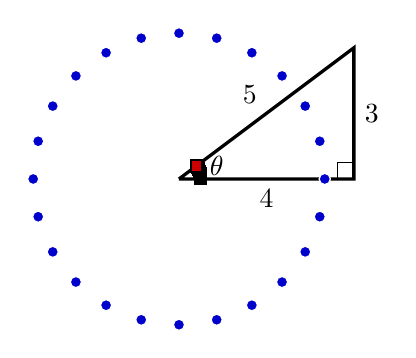
\begin{tikzpicture}
      \begin{axis}[xmax=1.2, axis equal=true, axis lines=none,
        width=2.75in, clip=false]
        \pgfmathsetmacro{\angle}{asin(3/5)};
        \addplot+[domain=0:360, white] ({cos(x)}, {sin(x)});
        \draw[very thick] (0,0) -- node[midway, below] {4} (1.2, 0) -- node[midway, right] {3} (1.2, 0.9) -- (0,0);
        \solonly{
        \draw[draw=none] (1.2,0.9) -- node[midway, above left] {5} (0,0);
        }
        \addplot+[domain=0:\angle, semithick, black] ({.15*cos(x)},
        {.15*sin(x)}) node[pos=0.5, anchor=200] {$\theta$};
        \draw (1.2, 0) rectangle ++(-6pt, +6pt);
      \end{axis}
    \end{tikzpicture}
\hspace{1in}
 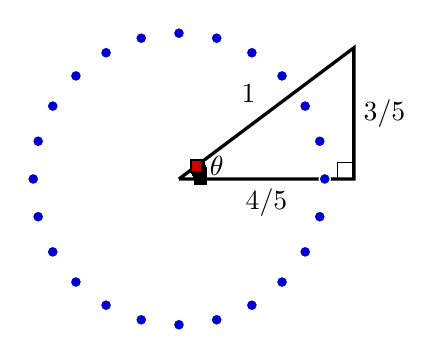
\begin{tikzpicture}
      \begin{axis}[xmax=1.2, axis equal=true, axis lines=none,
        width=2.75in, clip=false]
        \pgfmathsetmacro{\angle}{asin(3/5)};
        \addplot+[domain=0:360, white] ({cos(x)}, {sin(x)});
        \draw[very thick] (0,0) -- (1.2, 0) -- (1.2, 0.9) -- node[midway, above left] {1} (0,0);
        \solonly{
        \draw[draw=none] (0,0) -- node[midway, below] {4/5} (1.2, 0) -- node[midway, right] {3/5} (1.2, 0.9) -- (0,0);
        }
        \addplot+[domain=0:\angle, semithick, black] ({.15*cos(x)},
        {.15*sin(x)}) node[pos=0.5, anchor=200] {$\theta$};
        \draw (1.2, 0) rectangle ++(-6pt, +6pt);
      \end{axis}
    \end{tikzpicture}
\end{problem}

\begin{solution}
    We can use the Pythagorean theorem to determine that the missing side length in the triangle on the left is $5$. Then we can determine $\sin\theta$ by finding the ratio of the opposite side to the hypotenuse, $\frac{3}{5}$, and $\cos\theta$ by finding the ratio of the adjacent side to the hypotenuse, $\frac{4}{5}$.

    Since the triangle on the right has the same angles as the triangle on the left, the two triangles are similar. The hypotenuse has been scaled by a factor of $\frac{1}{5}$, so the other side lengths are correspondingly $\frac{3}{5}$ and $\frac{4}{5}$. The ratios of the opposite and adjacent sides to the hypotenuse, $\sin\theta$ and $\cos\theta$, remain the same.
\end{solution}

\item 
\begin{problem}
    Here is the same exact angle $\theta$ drawn in standard position on top of the unit circle. What are the values of $\sin\theta$ and $\cos\theta$? How do they show up in this diagram?

    \begin{tikzpicture}
      \begin{axis}[xmin=-1.2, xmax=1.4, axis equal=true, xtick={-1, 1}, ytick={-1,
          1}, width=2.75in,clip=true]
        \pgfmathsetmacro{\angle}{asin(3/5)};
        \addplot+[domain=0:360, semithick] ({cos(x)}, {sin(x)});
        \draw[very thick, ->] (axis cs: 0, 0) -- (axis
        cs: 1.2, 0.9);
        \draw[dashed] (axis cs: 0.8, 0.6) -- (axis cs: 0.8, 0);
        \addplot+[domain=0:\angle, semithick, black,->] ({.2*cos(x)},
        {.2*sin(x)}) node[pos=0.5, anchor=200] {$\theta$};
        \solonly{
        \addplot[closed] coordinates {(0.8,0.6)};
        \node[right] at (0.8,0.6) {$\big(\frac{4}{5},\frac{3}{5}\big)$};
        }
        \node[left] at (0.8,0.3) {$\frac{3}{5}$};
        \node[below] at (0.4,0) {$\frac{4}{5}$};
      \end{axis}
    \end{tikzpicture}
\end{problem}

\begin{solution}
    In the previous problem, we determined that in a right triangle with a hypotenuse of $1$ and angle $\theta$, the opposite leg to $\theta$ has a length of $\frac{3}{5}$ and the adjacent leg has a length of $\frac{4}{5}$. If we place this triangle on top of the unit circle with $\theta$ in standard position, this gives us the point $(\frac{4}{5}, \frac{3}{5})$ on the unit circle. So $\sin\theta$ is both the ratio of the opposite side to the hypotenuse, and the $y$-coordinate of the corresponding point on the unit circle. $\cos\theta$ is both the ratio of the adjacent side to the hypotenuse, and the $x$-coordinate of the corresponding point on the unit circle.
\end{solution}

\item
\begin{enumerate}
\item 
\begin{problem}
Sketch the angle $\pi-\theta$ in standard position on top of the unit circle. Why is it impossible to draw a right triangle that has this angle?
\end{problem}

\begin{solution}
The angle $\pi-\theta$ is more than $\pi/2$ and is thus obtuse, but a right triangle can never have an obtuse angle. The sum of the angles in a triangle must add to $\pi$ (\ang{180}), and since one of the angles is a right angle, the other two angles must add to $\pi/2$ (\ang{90}).
    \begin{center}
    \begin{tikzpicture}
      \begin{axis}[xmin=-1.2, xmax=1.4, axis equal=true, xtick={-1, 1}, ytick={-1,
          1}, width=2.75in,clip=true]
        \addplot+[domain=0:360, semithick] ({cos(x)}, {sin(x)});
        \draw[very thick, ->] (axis cs: 0, 0) -- (axis
        cs: -1.2, 0.9);
        \draw[dashed] (axis cs: -0.8, 0.6) -- (axis cs: -0.8, 0);
        \addplot+[domain=0:143.125, semithick, black,->] ({.2*cos(x)},
        {.2*sin(x)}) node[pos=0.5, anchor=200] {$\pi-\theta$};
        \solonly{
        \addplot[closed] coordinates {(-0.8,0.6)};
        }
      \end{axis}
    \end{tikzpicture}
    \end{center}
\end{solution}

\pspace{\vfill}

\item 
\begin{problem}
On the same picture, draw a vertical line segment from the terminal point on the unit circle down to the $x$-axis. This creates a \textbf{reference triangle}. Use the reference triangle to find $\sin(\pi-\theta)$ and $\cos(\pi-\theta)$.
\end{problem}
\pspace{\stretch{0.5}}

\begin{solution}
The reference triangle contains the same angle $\theta$ as before, so we know that the opposite side length is $\frac{3}{5}$ and the adjacent side length is $\frac{4}{5}$. Given the orientation of the triangle, we can thus determine that the coordinates of the terminal point on the circle are $(-\frac{4}{5}, \frac{3}{5})$. So $\sin(\pi-\theta)=\frac{3}{5}$, and $\cos(\pi-\theta)=-\frac{4}{5}$.
    \begin{center}
    \begin{tikzpicture}
      \begin{axis}[xmin=-1.2, xmax=1.4, axis equal=true, xtick={-1, 1}, ytick={-1,
          1}, width=2.75in,clip=true]
        \addplot+[domain=0:360, semithick] ({cos(x)}, {sin(x)});
        \draw[very thick, ->] (axis cs: 0, 0) -- (axis
        cs: -1.2, 0.9);
        \draw[dashed] (axis cs: -0.8, 0.6) -- (axis cs: -0.8, 0);
        \addplot+[domain=0:143.125, semithick, black,->] ({.2*cos(x)},
        {.2*sin(x)}) node[pos=0.5, anchor=200] {$\pi-\theta$};
        \solonly{
        \addplot[closed] coordinates {(-0.8,0.6)};
        \node[right] at (-0.8,0.6) {$\big({-\frac{4}{5}},\frac{3}{5}\big)$};
        \node[right] at (-0.8,0.3) {$\frac{3}{5}$};
        \node[below] at (-0.4,0) {$\frac{4}{5}$};
        \node at (\rtheta{0.4}{165}) {$\theta$};
        }
      \end{axis}
    \end{tikzpicture}
    \end{center}
\end{solution}
\end{enumerate}
\end{enumerate}


\end{enumerate}

\newpage


\begin{enumerate}[resume]

\item 
  \note{More practice with the symmetry of the unit circle.  (This tends
    to be a sticking point when we get to inverse trigonometric functions,
    so I want to try to prepare students as much as possible.) In
    particular, it's worthwhile to do {{{{\#3}}(g)}}.}

  If $\theta$ is the angle shown in the picture, evaluate each of the
  following.  (It will help to draw the angle in question on the unit
  circle and to use reference triangles.)

  \begin{tikzpicture}
    \begin{axis}[xmin=-1.2,xmax=1.2,ymin=-1.2,ymax=1.2,
    width=3in, unit vector ratio*={1 1},
    xtick={-1,1}, ytick={-1,1},clip=false,
    x tick label style = {xshift = 6pt},
    y tick label style = {yshift = 6pt}]
    \coordinate (O) at (0,0);
    \coordinate (A) at (1,0);
    \coordinate (B) at (5/13,12/13);
    \addplot[black,domain=0:360,data cs=polar] (x,1);
    \draw (O) -- (B) node[above right]
    {$\displaystyle \left( \frac{5}{13}, \frac{12}{13} \right)$};
    \draw pic[draw=black, angle radius=10, "$\theta$",
    angle eccentricity = 1.8, ->] {angle=A--O--B};
    \filldraw[radius=2pt] (B) circle;
    \end{axis}
  \end{tikzpicture}
  
  \vspace{6pt}

  \probonly{
  \begin{tasks}(4)
      \task 
      \begin{problem}
      $\sin \theta$
    \end{problem}

    \task 
      \begin{problem}
      $\sin (-\theta)$
    \end{problem}

    \task 
      \begin{problem}
      $\cos \theta$
    \end{problem}

    \task 
      \begin{problem}
      $\cos(-\theta)$
    \end{problem}

  \end{tasks}
  }
  \pspace{\vfill}

  \begin{enumerate}
  \item
    \begin{problem}
      $\sin \theta$
    \end{problem}

    \begin{solution}
      $\sin \theta$ is the $y$-coordinate of the terminal point,
      which is $\boxed{\frac{12}{13}}$. We can drop a vertical line segment to the $x$-axis to get a triangle which will be useful in the following parts.
      \begin{center}
        \begin{tikzpicture}
    \begin{axis}[xmin=-1.2,xmax=1.2,ymin=-1.2,ymax=1.2,
    width=3in, unit vector ratio*={1 1},
    xtick={-1,1}, ytick={-1,1},clip=false,
    x tick label style = {xshift = 6pt},
    y tick label style = {yshift = 6pt}]
    \coordinate (O) at (0,0);
    \coordinate (A) at (1,0);
    \coordinate (B) at (5/13,12/13);
    \addplot[black,domain=0:360,data cs=polar] (x,1);
    \draw (O) -- (B) node[above right]
    {$\displaystyle \left( \frac{5}{13}, \frac{12}{13} \right)$};
    \draw pic[draw=black, angle radius=10, "$\theta$",
    angle eccentricity = 1.8, ->] {angle=A--O--B};
    \filldraw[radius=2pt] (B) circle;
    \draw[dashed] (B) -- node[midway, right] {$\frac{12}{13}$} (B|-O) -- node[midway, below] {$\frac{5}{13}$} (O);
    \end{axis}
  \end{tikzpicture}
  \end{center}
    \end{solution}

  \item
    \begin{problem}
      $\sin(-\theta)$
    \end{problem}

    \begin{solution}
      When we draw in the angle $- \theta$, dropping a vertical line segment to the $x$-axis gives us the same reference triangle as before, with the exact same lengths. We can use these lengths to determine that the coordinates of the terminal point are $\left(
        \frac{5}{13}, -\frac{12}{13} \right)$, so $\sin ( - \theta) =
      \boxed{-\frac{12}{13}}$.
      \begin{center}
  \begin{tikzpicture}
    \begin{axis}[xmin=-1.2,xmax=1.2,ymin=-1.2,ymax=1.2,
    width=3in, unit vector ratio*={1 1},
    xtick={-1,1}, ytick={-1,1},clip=false,
    x tick label style = {xshift = 6pt},
    y tick label style = {yshift = 6pt}]
    \coordinate (O) at (0,0);
    \coordinate (A) at (1,0);
    \coordinate (B) at (5/13,-12/13);
    \addplot[black,domain=0:360,data cs=polar] (x,1);
    \draw (O) -- (B) node[below right]
    {$\displaystyle \left(\frac{5}{13}, -\frac{12}{13} \right)$};
    \draw pic[draw=black, angle radius=5, "$-\theta$",
    angle eccentricity = 2.8, ->] {angle=B--O--A};
    \draw[dashed] (B) -- node[midway,right] {$\frac{12}{13}$} (B|-O) -- node[midway, above] {$\frac{5}{13}$} (O);
    \filldraw[radius=2pt] (B) circle;
    % \node at (\rtheta{0.15}{330}) {$\theta$};
    \end{axis}
  \end{tikzpicture}
      \end{center}
    \end{solution}

  \item
    \begin{problem}
      $\cos \theta$
    \end{problem}

    \begin{solution}
      $\cos \theta$ is the $x$-coordinate of the terminal point,
      which is $\boxed{\frac{5}{13}}$. 
    \end{solution}

  \item
    \begin{problem}
      $\cos(-\theta)$
    \end{problem}

    \begin{solution}
     Referring to our previous diagram for $-\theta$, the coordinates of the terminal point are $\left(
        \frac{5}{13}, -\frac{12}{13} \right)$, so $\cos ( - \theta) =
      \boxed{\frac{5}{13}}$.
    \end{solution}

\item
    \begin{problem}[1.25in]
      $\cos (\pi + \theta)$
    \end{problem}

    \begin{solution}
      The angle $ \pi + \theta$ is shown. We have the exact same reference triangle as before, just in a different orientation. The terminal point has coordinates $\left(-\frac{5}{13}, -
        \frac{12}{13} \right)$, so $\cos (\pi + \theta) =
      \boxed{-\frac{5}{13}}$. 
      \begin{center}
  \begin{tikzpicture}
    \begin{axis}[xmin=-1.2,xmax=1.2,ymin=-1.2,ymax=1.2,
    width=3in, unit vector ratio*={1 1},
    xtick={-1,1}, ytick={-1,1},clip=false,
    x tick label style = {xshift = 6pt},
    y tick label style = {yshift = 6pt}]
    \coordinate (O) at (0,0);
    \coordinate (A) at (1,0);
    \coordinate (B) at (-5/13,-12/13);
    \addplot[black,domain=0:360,data cs=polar] (x,1);
    \draw (O) -- (B) node[below left]
    {$\displaystyle \left(-\frac{5}{13}, -\frac{12}{13} \right)$};
    \draw pic[draw=black, angle radius=5, 
    angle eccentricity = 2.8, ->] {angle=A--O--B};
    \draw[dashed] (B) -- node[midway,left] {$\frac{12}{13}$} (B|-O) -- node[midway, above] {$\frac{5}{13}$} (O);
    \filldraw[radius=2pt] (B) circle;
    \node at (\rtheta{0.3}{45}) {$\pi + \theta$};
    \end{axis}
  \end{tikzpicture}
      \end{center}
      
    \end{solution}

  \item
    \begin{problem}[1.25in]
      $\sin (2 \pi - \theta)$
    \end{problem}

    \begin{solution}
      The angle $2 \pi - \theta$ is shown. We again have the exact same reference triangle as before, just in a different orientation. The terminal point has coordinates $\left( \frac{5}{13}, -
        \frac{12}{13} \right)$, so $\sin (2 \pi - \theta) =
      \boxed{-\frac{12}{13}}$. 
      \begin{center}
  \begin{tikzpicture}
    \begin{axis}[xmin=-1.2,xmax=1.2,ymin=-1.2,ymax=1.2,
    width=3in, unit vector ratio*={1 1},
    xtick={-1,1}, ytick={-1,1},clip=false,
    x tick label style = {xshift = 6pt},
    y tick label style = {yshift = 6pt}]
    \coordinate (O) at (0,0);
    \coordinate (A) at (1,0);
    \coordinate (B) at (5/13,-12/13);
    \addplot[black,domain=0:360,data cs=polar] (x,1);
    \draw (O) -- (B) node[below right]
    {$\displaystyle \left(\frac{5}{13}, -\frac{12}{13} \right)$};
    \draw pic[draw=black, angle radius=5, "$2\pi-\theta$",
    angle eccentricity = 2.8, ->] {angle=A--O--B};
    \draw[dashed] (B) -- node[midway,right] {$\frac{12}{13}$} (B|-O) -- node[midway, above] {$\frac{5}{13}$} (O);
    \filldraw[radius=2pt] (B) circle;
    \end{axis}
  \end{tikzpicture}
      \end{center}
      
    \end{solution}
    \end{enumerate}

    \probonly{
    \begin{tasks}[start=5](4)
        \task 
    \begin{problem}
      $\cos (\pi + \theta)$
    \end{problem}

    \task
    \begin{problem}
      $\sin (2 \pi - \theta)$
    \end{problem}
        \task
        \begin{problem}
        $\cos (2 \pi + \theta)$
        \end{problem}

        \task
        \begin{problem}
        $\sin (2\pi + \theta)$
        \end{problem}
    \end{tasks}
    }
    \pspace{\vfill}

    \solonly{
    \begin{enumerate}
  \item
    \begin{problem}
      $\cos (2 \pi + \theta)$
    \end{problem}

    \begin{solution}
      The angle $2 \pi + \theta$ ends in the same place that $\theta$
      does:
      \begin{center}
        \begin{tikzangle}[angle=rad(acos(5/13)), xtick={-1, 1}, ytick={-1,
            1}, width=2.5in, height=2.5in, clip=false, color=black]
          \pgfmathsetmacro{\new}{2*pi+\angle};
          \addplot+[domain=0:\new, red, thin, ->, >=to] ({0.15*1.05^x*cos(deg(x))},
          {0.15*1.05^x*sin(deg(x))});
          \filldraw (axis cs: \px, \py) circle(1.5pt) node[anchor=\anchor]
          {$\displaystyle \left( \frac{5}{13}, \frac{12}{13} \right)$};
          \draw[red] (axis cs: 0, 0) -- (axis cs: \px, \py);
          \filldraw[red] (axis cs: \px, \py) circle(1.5pt);
        \end{tikzangle}
      \end{center}
      So, $\cos (2 \pi + \theta) = \boxed{\frac{5}{13}}$.
    \end{solution}

      \item
    \begin{problem}
      $\sin (2 \pi + \theta)$
    \end{problem}

    \begin{solution}
      The angle $2 \pi + \theta$ ends in the same place that $\theta$
      does:
      \begin{center}
        \begin{tikzangle}[angle=rad(acos(5/13)), xtick={-1, 1}, ytick={-1,
            1}, width=2.5in, height=2.5in, clip=false, color=black]
          \pgfmathsetmacro{\new}{2*pi+\angle};
          \addplot+[domain=0:\new, red, thin, ->, >=to] ({0.15*1.05^x*cos(deg(x))},
          {0.15*1.05^x*sin(deg(x))});
          \filldraw (axis cs: \px, \py) circle(1.5pt) node[anchor=\anchor]
          {$\displaystyle \left( \frac{5}{13}, \frac{12}{13} \right)$};
          \draw[red] (axis cs: 0, 0) -- (axis cs: \px, \py);
          \filldraw[red] (axis cs: \px, \py) circle(1.5pt);
        \end{tikzangle}
      \end{center}
      So, $\sin (2 \pi + \theta) = \boxed{\frac{12}{13}}$.
    \end{solution}

 
    \end{enumerate}}

\begin{enumerate}[start=9]
\item
\begin{problem}
    Evaluate $(\sin \theta)^2 + (\cos \theta)^2$ (also written $\sin^2 \theta + \cos^2\theta$). Is the value you get a coincidence?
\end{problem}
\pspace{\stretch{0.5}}

\begin{solution}
    \begin{align*}
        \sin^2 \theta + \cos^2 \theta &= \left(\frac{12}{13}\right)^2 + \left(\frac{5}{13}\right)^2 \\
        &= \frac{144}{169} + \frac{25}{169} \\[4pt]
        &= 1
    \end{align*}
    This is not a coincidence, as we know that the coordinates $\left(
        \frac{5}{13}, \frac{12}{13} \right)$ are a point on the unit circle and thus must satisfy $x^2+y^2=1$. The particular value of $\theta$ did not matter here, so we can deduce that, no matter the value of $\theta$,
        \[\sin^2\theta+\cos^2\theta=1\]
        which is called the Pythagorean Identity.
\end{solution}

  \end{enumerate}

\item
Some facts about sine and cosine are true for \emph{any angle}. We call these facts \textbf{identities}. Which of the following are true identities? Use the unit circle to help you decide.

\probonly{
\begin{tasks}[after-item-skip=24pt, after-skip=24pt](2)
    \task $\sin(-\theta)=-\sin(\theta)$
    \task $\cos(-\theta)=-\cos(\theta)$
    \task $\sin\theta + \cos\theta =1$
    \task $\sin^2 \theta + \cos^2\theta = 1$
    \task $\sin(\theta+2\pi)=\sin\theta$
    \task $\cos(\theta+2\pi) = \cos\theta$
\end{tasks}
}

\solonly{
\begin{enumerate}
    \item 
    \begin{problem}
        $\sin(-\theta)=-\sin(\theta)$
    \end{problem}

    \begin{solution}
        This is always true. In standard position, the angle $\theta$ and $-\theta$ are vertical reflections of each other over the $x$-axis. Thus, the $y$-coordinate corresponding to $\theta$ and the $y$-coordinate corresponding to $-\theta$ will always be opposites, $\sin(-\theta) = -\sin(\theta)$.
    \end{solution}

        \item 
    \begin{problem}
        $\cos(-\theta)=-\cos(\theta)$
    \end{problem}

    \begin{solution}
        This is not a true identity. In standard position, the angle $\theta$ and $-\theta$ are vertical reflections of each other over the $x$-axis. Thus, the $x$-coordinate corresponding to $\theta$ and the $x$-coordinate corresponding to $-\theta$ will always be the same, not opposites, $\cos(-\theta) = \cos(\theta)$.
    \end{solution}

        \item 
    \begin{problem}
        $\sin\theta + \cos\theta =1$
    \end{problem}

    \begin{solution}
        This is not a true identity. We can check one value of $\theta$ to disprove it. For $\theta=\pi$, $\sin\pi + \cos\pi = 0 + (-1) = -1$.
    \end{solution}

        \item 
    \begin{problem}
        $\sin^2 \theta + \cos^2\theta = 1$
    \end{problem}

    \begin{solution}
        This is always true, because the $\sin\theta$ and $\cos\theta$ can be thought of as the coordinates of a point on the unit circle, and the $x$- and $y$-coordinates of a point on the unit circle must satisfy $x^2+y^2=1$.
    \end{solution}

        \item 
    \begin{problem}
        $\sin(\theta+2\pi)=\sin\theta$
    \end{problem}

    \begin{solution}
        This is always true. The angle $\theta + 2\pi$ is coterminal with $\theta$, so the terminal point will have the same exact coordinates.
    \end{solution}

        \item 
    \begin{problem}
        $\cos(\theta+2\pi) = \cos\theta$
    \end{problem}

    \begin{solution}
        Always true, for the same reason as the last part. 
    \end{solution}
\end{enumerate}
}
  
\end{enumerate}

\end{document}